%!TEX encoding = MacOSRoman
%!TEX TS-program = xelatex
%!BIB TS-program = bibtex

% --------------------- Start of Document Preamble -----------------------

\documentclass[12pt, oneside]{report} % report is suitable for the long document such as Ph.D thesis with chapters
\usepackage[a4paper, left=1in, right=1in, top=1in, bottom=1in]{geometry} 
\usepackage{fontspec}
\setmainfont{Times New Roman}
\usepackage{pdflscape}
\usepackage{apacite}
%\usepackage[round]{natbib}  % the bibliography
\usepackage{sectsty}
\chapterfont{\centering}
\usepackage{enumitem} % enumerate package
\linespread{2}
\usepackage{amsmath,amssymb,amstext} % Lots of math symbols and environments
\usepackage{graphicx} % For including graphics N.B. pdftex graphics driver 

%----- Adjust the style ----
\renewcommand{\chaptername}{CHAPTER}
\renewcommand{\thechapter}{\Roman{chapter}}
% ---------------------- End of Document Preamble ------------------------

%======================================================================
%   L O G I C A L    D O C U M E N T -- the content of your thesis
%======================================================================
\begin{document}

% For a large document, it is a good idea to divide your thesis
% into several files, each one containing one chapter.
% To illustrate this idea, the "front pages" (i.e., title page,
% declaration, borrowers' page, abstract, acknowledgements,
% dedication, table of contents, list of tables, list of figures,
% included into the document by the following statement.
%----------------------------------------------------------------------
% FRONT MATERIAL
%----------------------------------------------------------------------
% T I T L E   P A G E
% -------------------
% Last updated May 24, 2011, by Stephen Carr, IST-Client Services
% The title page is counted as page `i' but we need to suppress the
% page number.  We also don't want any headers or footers.
\pagestyle{empty}
\pagenumbering{roman}

% The contents of the title page are specified in the "titlepage"
% environment.
\begin{titlepage}
        \begin{center}
        \vspace*{0.5cm}

        \normalsize
        {\bf NETWORK ANALYSIS OF RICE HEALTH SUREVEY DATA FOR CHARACTERIZATION OF YIELD REDUCING FACTORS AND YIELD LIMITING FACTORS OF TROPICAL RICE ECOSYSTEM IN SOUTH AND SOUTHEAST ASIA}

        \vspace*{4.0cm}

        \normalsize
        \bf{SITH JAISONG} \\

        \vspace*{4.0cm}

        \normalsize
        THESIS OUTLINE SUBMITTED TO THE FACULTY OF GRADUATE SCHOOL\\
        UNIVERSITY OF THE PHILIPPINES LOS BA~{N}OS\\ 
 IN FULFILLMENT OF THE \\
        REQUIREMENT FOR THE \\ 
        DEGREE OF \\
        \vspace*{2.0cm}
        PH.D OF SCIENCE \\
        (Plant Pathology) \\

        \vspace*{1.0cm}
%        \copyright\ Pat Neugraad 2007 \\
        May 2015
        \end{center}
\end{titlepage}

% The rest of the front pages should contain no headers and be numbered using Roman numerals starting with `ii'
\pagestyle{plain}
\setcounter{page}{2}

\cleardoublepage % Ends the current page and causes all figures and tables that have so far appeared in the input to be printed.
% In a two-sided printing style, it also makes the next page a right-hand (odd-numbered) page, producing a blank page if necessary.
 
%------------Setting the bibliography style --------------



%------------End of the bibliography style ----------------

% D E C L A R A T I O N   P A G E
% -------------------------------
  % The following is the sample Delaration Page as provided by the GSO
  % December 13th, 2006.  It is designed for an electronic thesis.
%  \noindent
%I hereby declare that I am the sole author of this thesis. This is a true copy of the thesis, including any required final revisions, as accepted by my examiners.

%  \bigskip
  
%  \noindent
%I understand that my thesis may be made electronically available to the public.

%\cleardoublepage
%\newpage

% A B S T R A C T
% ---------------

%\begin{center}\textbf{Abstract}\end{center}

% You're not characterizing different environments. They're all tropical, irrigated, lowland rice
%Characterising rice agroecosytems requires knowledge and information of qualitative and quantitative information. One way of gathering data the data necessary for this is through the conduct of surveys. Given the nature of the data, it is not a simple task to analyse and examine in order to derive information and knowledge. One method in particular, network analysis, has been used to explore the observed relationships between the individual elements in a given system. This study is the first known attempt to apply network analysis to the analysis of in-field and household survey data on rice yield limiting and reducing factors. The data will be analyzed and visualized using the proposed network model. I propose to construct a network model using survey data collected from 2009 to 2011 in several sites (Chekempek, West Java, Indonesia; Mekong River Delta, Vietnam; Tamil Nadu, India; and Suphaburi, Thailand) and test the model with data collected from 2012 to 2015 in several cropping seasons and sites (Chekempek, West Java, Indonesia; Red River Delta, Vietnam; Tamil Nadu and Odisha, India; Suphaburi, Thailand). The anticipated results from this research will be helpful for plant health authorities worldwide, in order to design specific strategies for rice pest and disease management and to limit the impacts of these yield reducing factors. 


%\cleardoublepage
%\newpage

% A C K N O W L E D G E M E N T S
% -------------------------------

%\begin{center}\textbf{Acknowledgements}\end{center}

%I would like to thank all the little people who made this possible.
%\cleardoublepage
%\newpage

% D E D I C A T I O N
% -------------------

%\begin{center}\textbf{Dedication}\end{center}

%\cleardoublepage
%\newpage

% T A B L E   O F   C O N T E N T S
% ---------------------------------
\renewcommand\contentsname{TABLE OF CONTENTS}
\tableofcontents
\cleardoublepage
%\phantomsection
%\newpage

% L I S T   O F   T A B L E S
% ---------------------------
%\addcontentsline{toc}{chapter}{List of Tables}
%\listoftables
%\cleardoublepage
%\phantomsection		% allows hyperref to link to the correct page
%\newpage

% L I S T   O F   F I G U R E S
% -----------------------------
\addcontentsline{toc}{chapter}{LIST OF FIGURES}
\listoffigures
\cleardoublepage
%\phantomsection		% allows hyperref to link to the correct page
%\newpage

% L I S T   O F   S Y M B O L S
% -----------------------------
% To include a Nomenclature section
% \addcontentsline{toc}{chapter}{\textbf{Nomenclature}}
% \renewcommand{\nomname}{Nomenclature}
% \printglossary
% \cleardoublepage
% \phantomsection % allows hyperref to link to the correct page
% \newpage

% Change page numbering back to Arabic numerals
\pagenumbering{arabic}
 

%----------------------------------------------------------------------
% MAIN BODY
%----------------------------------------------------------------------
% Because this is a short document, and to reduce the number of files
% needed for this template, the chapters are not separate
% documents as suggested above, but you get the idea. If they were
% separate documents, they would each start with the \chapter command, i.e, 
% do not contain \documentclass or \begin{document} and \end{document} commands.

%======================================================================
% INTRODUCTION
\chapter{INTRODUCTION}
%======================================================================
%=========================
%INTRODUCTION
%=========================
%\section*{Introduction}
\addcontentsline{toc}{chapter}{Introduction}
% 1. Threats do not reduce yields. Pests and diseases do. Rewrite.
% 2. Cite Oerke for actual and potential losses to bolster your case.
% 3. Your second sentence is out of place with the opening. You need to work on making the paragraph flow.
% 4. I'd argue that it's important for not just rice consuming societies but globally due to the interconnectedness of our modern societies.
The threats of pests and diseases to global rice production are significant yield reducing factors. Additionally, future rice production will need to grow by 2.4\% per year in order to meet the demands of a growing population \shortcite{Ray:2013by}. Addressing these yield-reducing factors is essential for food security in rice consuming societies now and in the future. 

% first sentence is incomprehensible
% the second sentence is an incomplete thought, untie what?
% grammar in the third sentence
% fourth sentence, if they have not been insufficient then why would you do this? Obviously they succeeded
% season is a noun, not an adjective
Description of pest management is complicated because human activities regarding with agricultural practices to the pests are diverse. To achieve this, the knowledge of relationships between pests and human activities including environmental factors are needed to untie \shortcite{Savary:2000ws}. While these studies are important in characterization the of pattern of pest injuries and the pattern of components relating to production situation, and how it related to each others. They have not been insufficient for explanation about change of relationships of injuries and components of production situation in term of time and regions, or how such relationships may change with climate variations.  For instance, the  relations between insect pest and weed were found only in the certain time, or certain locations. Over the long run, in season correlation between the frequency of patterns of pest incidence at different locations are also important to design the pest management strategies.

% this paragraph seems out of place with the first two. You need to work on flow. Your opening sentence should really be something more like your second sentence here.
We live in an increasingly connected era where by early 2013 over 90\% of all data had been generated to that point \shortcite{SINTEF}. In agriculture we should strive to find ways to harness our own ''big data''. We have a daunting task ahead of us that will require a myriad of approaches from well-know and understood to new approaches like big data analytics. Using new approaches to analyze so called ``big data'', we can start making new discoveries in relationships between factors of which we were previously unaware. These newly discovered relationships could be useful in designing and developing methods for managing plant pests and diseases.

% Ok, introducing network models. Good, but you need to give a bit more background first on some of the other methods too, this is just too blunt. You have a space before a "."
Network models provide powerful tools in many branches of science, which are applied for generate to . A network is an abstract model composed of a set of nodes or vertices, a set of edges, links or ties that connect the nodes, together with information concerning the nature of the nodes and edges. The nodes usually represent entities and the edges represent their relations. This simple model can be used to describe many kinds of phenomena, such as social relations, technological and biological structures, and information networks.
%-----------------------------
\section*{OBJECTIVES}
%----------------------------

% 1. Rethink the use of the idea of yield "constraints". Also, for the last time, constrain is a VERB. Constraint is a noun. Learn it. Apply it. Use it. Never make the mistake ever again even though you won't be using the term in this context because I told you to rethink it. 
% 1a. The opening sentence makes no sense even if yield constraints were the proper terminology to use.
% 2. Are you sure about addressing how pests and cropping practices relate to yields?
% 3. The third sentence is poorly written and not easily understood.
% 4. The last sentence is incomprehensible. 
% 4a. "The examples"? You are indicating that the examples you have are THE only examples possible. Think back to the in-depth conversation with you about the use of the word "the" when describing things like this and how you should use it.

% Lastly, I don't agree with your "objectives" as you've written them here.
My objectives are to synthesize approaches to characterize the yield constrains under agroecosystem. I also address how pests and cropping practices relate to yields individually and simultaneously. For better understanding, climatic variable can be possibly added. Finally, I propose the examples of new applications and a conceptual framework for exploring the relationships of injuries caused by pests, human activities under different geographic location.

% I see three questions? Which one are you answering of the following?
The networks constructed will attempt to answer the following question. 
\begin{enumerate}

\item How can the rice yield losses be examine from the perspective of networks analysis. What the key factors affect to rice yield productivities? and how variation is in different locations?  
\item What relationships between components of networks as defined in the variables in survey profile data? 
% why is the there a space before the "?"?
\item How are theses relationships affects by different locations ?

\end{enumerate}
% 1. The anticipation of the proposed work won't provide anything other than that, anticipation. Rewrite.
% 2. Second sentence is incomprehensible. Rewrite.
% 3. Third sentence is  incomprehensible. Rewrite.
The anticipation of the proposed work will provide the insights of rice injuries from network inference of rice crop health survey data. Complete an analysis of the crop health survey data using the new network model and provide visualizations and interpretations of the results and make rice crop health recommendations based on findings. It will be very helpful for plant health authorities worldwide, in order to design specific strategies for rice pest and disease management and to limit the impacts of these yield reducing factors.
 



\chapter{REVIEW OF LITERATURE}
%====================================
% introduction of literature review
%===================
\section*{Introduction}
%==================
\label{ch:intro}

The applications of network analysis have increased exponentially over the past two decades in various disciplines. Even though documented applications of network analysis in plant pathology are still relatively sparse, network applications in the social science, systems biology and ecology have been increasingly found. \shortciteA{Shaw:2014cka, MoslonkaLefebvre:2011fo, Jeger:2007tn, windram2014network} presented useful concepts and methods of network analysis in the studies related to plant pathology. I review the empirical works that exist and argue that network analysis is a promising approach for exploring the questions in the context of plant pathology.

This chapter contains four sections of review of network analysis and its applications. In the first sections, I introduces a brief overview of the concepts and methods of network analysis. I then discuss the new dimensions of network analysis that are not found in other approaches. In the first two sections, I provide an overview of key of network concepts and place network analysis as a methodology within the broader toolbox of methods commonly used in biological studies.
  

In the third section I scope network analysis  into the current applications of plant pathological research, particularly in plant disease epidemiology and molecular plant pathology, in which network analysis has been broadly applied, and increasingly documented. It provides fruitful tools for visualizing, analyzing and understanding complex relationships in the studies of plant disease. For instance, network models of genes or proteins pertaining plant defense mechanism and network models revealing spatial distribution of plant disease through trade networks were reviewed by \shortciteA{windram2014network} and \shortciteA{Shaw:2014cka} respectively. 

The last section presents analytical techniques and strategies to apply network analysis for studying pest management. It introduces three strategies of network applications, which are developed and applied in the studies of systems biology and ecology, and concludes the brief discussions of potential applications to the studies of crop heath management that have yet been undertaken.

\section*{PartI: Network Analysis}
%==========================
\label{ch:partone}

\subsubsection{Introduction to network analysis}
Network analysis is applied for determining relationships between elements of interest. It offers toolkits for visualizing data in a network model and measuring its properties, and network thinkings \shortcite{PROULX:2005hx}. It been widely used by various branches of science, such as social science, ecology, biology, computer science, and many others to study the interactions between elements, e.g., the relationships of students in school \shortcite{moody2001race}, species in food webs \shortcite{krause2003compartments}, interactions of genes or proteins in cells \shortcite{guimera2005functional}, or the connections of computer in the network \shortcite{pastor2001epidemic, newman2006modularity}.

\shortciteA{newman2003structure} loosely categorized four types of networks based on different complex data. The first category is social network, representing sets or groups of people forming some patterns of contacts or interactions between them such as the patterns of friendship or business relationships. Analyzing the structure of whole social entities gives us the perspectives from a social network, which enables us to explain the patterns observed. \shortciteA{moody2001race} analyzed the social behaviors in high school students using social network approaches. \shortcite{Kasari2011s} applied network analysis to compare the social relationships and friendships between children with and without Autism spectrum disorder (ADS). The second type of network is an information network or knowledge network. The classic example of this network is the network of citations between academic papers \shortcite{newman2003structure}. The articles cited other papers, which have related topics. They formed a citation network that has vertices as articles and direct links as citations. The citation network visualizes the structure and the movement of the information. The third category, technological network, is object connected network, or man--made network which represents a physical connection between objects. This network is mostly applied for illustrating physical structures and systems such as the electrical power grid, the connections of rivers, transport systems, etc. The fourth category of network is a biological network. It represents the biological systems such as genes to genes, genes to protein, protein to protein interactions, which enable biologists understand the connections and interactions between individual constituents including genes, proteins, and metabolites at the level of the cell, tissue and organ to ultimately describe the entire organism system. Biologists use biological networks in various branches of biology at different levels (from a single molecule to an entire organism). For example, \shortcite{yang2014gene, barabasi2004network} studied in the patterns of gene expression in different conditions and different types of cells (normal cells and cancer cells) in order to characterize the genes that change and do not change following the particular conditions; \shortcite{freilich2010large} applied a molecular ecological network analysis to study the communities of soil microorganisms. Networks revealed the complex relationships between microbial species in soils and their communities. Moreover, network analysis enables ecologists to understand ecological properties and predict the ecological roles of species in a soil ecosystem. Although the application of each type of network approach varies, all four categories of networks share a common empirical focus on relational structure and a similar set of mathematical analysis. 

% add more the ecological studies related to plant disease
In plant pathological studies network analysis can be the powerful tool to study plant disease epidemics. \shortciteA{MoslonkaLefebvre:2011fo} showed the  the potential for the use of network analysis in plant epidemiology. Network analysis can reveal the dynamics of the disease spread. The theory and tools of network analysis support plant pathological studies. \shortciteA{MoslonkaLefebvre:2011fo} reviewed the studies related to plant disease which applied network analysis. Networks applied in the studies of plant disease are generally similar to ecological studies. In plant pathology, most network analysis is used in molecular plant pathology as a model of the interactions between genes and/or proteins, and other cellular constituents contributing to host plant resistance or pathogen infection. Spatial analysis 


\subsection*{Concepts, principles, and methods of network analysis}

A network represents relationships between of elements of interests, which is defined by links (edges) among nodes (vertices). Nodes can be units of interests or studies, and links represent interactions between nodes. Network analysis aims the association among nodes rather than the attributes of particular nodes. In network analysis, networks are defined as any set or set of links between any set or sets of nodes.


Network analysis follows three principles. Nodes and their behaviors are mutually dependent, not autonomous; links between nodes can be channels for transmission of both material (for example, money, disease) and non-material (for example, information, knowledge, relationship, interaction) and; persistent pattern of association among nodes create structure that can define, enable, or restrict the behavior of a node.  

Network models have two different organizational structures depending on the goal of the representation and analysis \shortcite{borgatti2013analyzing}. Flow models view the network as a system of pathways along which things flow between nodes. Analysis of flow models can, for example, identify which nodes in the network are more active, or which ones are more powerful. Flow models are good for evaluating processes, as was shown in these reviews of plant disease spread \shortcite{Jeger:2007tn, Shaw:2014cka}. Architectural models tend to focus on the structure of the network, seeking to discern whether specific structures lead to similar outcomes, or whether actors in similar network positions behave in similar ways. Ecological applications related to the ecology and spatial structure of ''community'' tend to be organized and analyzed as architectural models. For example, \shortciteA{Faust:2012dk} studied the networks of soil microbial interactions. Network models describes how microbial populations change over time, which will require the use of dynamic models of microbial communities. Beyond these basic principles, network analysis enables the calculation of structural properties of nodes, groups, or the entire network.

\textit{Measuring network properties}


A network is made up of nodes and links from relational data. It is constructed from adjacency matrix, which is obtained from analysis using metric algebra techniques. The row and column headings for an adjacency matrix are identical, listing the names of the components involved in the network. In the simplest case, the cells of the matrix are coded with ''1'' if an link exists between the node or ''0'' if no edge exists. However, a link can be valued. Value indicates a characteristic of the relationship that the research has quantified. The values may be binary, such as whether two friends recognize each other, or variable strength, e.g., the number of mutual friends between two friends. Network link need not to imply positive or cooperative interaction; they can also be negative or competitive interaction between two individuals.    


The distribution of links in a network suggests two important structural characteristics: centrality (importance) of nodes in the network and division of the network into subgroups. Variants of centrality in a network include degree, closeness, and betweenness. Degree centrality of a node is the sum of the value of the links between that node and every other node in the network. This measure tells us how well-connected a particular node is to the other nodes. Closeness centrality is calculated using the length of the path between a node and every other node. This measure could estimate the time required for information or resources to propagate to a given node in a network. Betweenness centrality corresponds to the number of paths in the network that pass through a particular node, and therefore measures the dependence of a network on a particular node for maintaining connectedness \shortcite{Toubiana:2013cv}. \shortciteA{Deng:2012do, newman2003structure, Toubiana:2013cv} are recommended references for descriptions of the theory and uses, as well as the formal calculation of these measures.


 %==========================
\section*{Part II: The dimensions of network analysis unlike other approaches}
%==========================
\label{parttwo}

%There are four key points to consider in network analysis :
%1) how does it differ from traditional approaches to social science research; 
%2) how does it relate to those traditional approaches; 
%) how are networks are constructed, manipulated and measured; and 
%4) what is value of network offers beyond traditional approaches.

With an increasing trend towards a systems level perspective in the science, away from the reductionism that characterized much of the previous century \shortcite{kolaczyk2014statistical}, the development of network analysis challenges conventional approaches to uncover the complex patterns of interaction or relationships. 

The difference of network analysis from conventional approaches is that it involves different methods of analysis. 
Network analysis models the relational data, and measures various properties of network. A challenge of network analysis is the consideration of the properties of interactions  between elements in the system, which interactions are assumed that they are dependent on each other. That is, when element A has a relationship with element B, the relationship is not only considered to be independent of element A and B, but also relationship of element A and B to be independent to other element. Unlike network analysis, traditional research methods consider attributes such as variables in a wide variety of statistical analyses, these methods are sometimes referred to as variable analysis \cite{scott2012social}.

As objects for representing interactions among elements of a complex system, network graphs are primarily focused in network analysis. Interactions or relationships are represented as edges in networks. They present only when interactions are exist between nodes. Moreover, network concepts place nodes in rational distance according to the level of relationships. For example, to visualize the strong relationship of A and B, network places the node represented A near the node represented B. Here is the new dimensions network of visualizing interactions or relationships.
 
Extending from considering the interaction of two nodes, network graphs illustrate nicely the connections. when node A relates to node B, and to the node C are found relationships, the network graph is able to visualize the connection between node A to node B, and to node C. This pattern, so-called "betweenness", potentially is useful to represent what the important node is in network graph because node A has high connectivity and is a connector between node B and node C. For example, In protein-protein interaction (PPI) network, proteins with high betweenness have been termed "bottlenecks", for their role as key connector proteins with essential functional and dynamic properties \shortcite{barabasi2011netmed}.

The heart of network study is structure; network processes replace vertices and edges in rational spaces depending on the selected graph layout methods. The network structure enable scientists to study interactions with behaviors and attributes of pairs of vertices. Networks would reveal the groups of vertices, which are closely related or similar to each other. This is also similar to the basis for the cluster analysis. For example, if the employees of the same company may share similar attributes such as location or educational background and they are close in network. When the relationships are simple and the differences in node attributes are clear, the conventional analytic approaches such as cluster analysis, principal component analysis, correspondence analysis are sufficient. However, when relationships are complex or vertices attributes are more nuanced, clear answers using conventional analysis may prove elusive. Network analysis offers a tool to help researchers disentangle some of the relational complexities.

\section*{Part III: Network and botanical epidemiology}
\label{ch:partthree}

Recently, a broad expansion in the use of network analysis has occurred across many disciplines over the past decade, and several researchers have evaluated the impact and potential of network approach on their respective disciplines. Networks are considered into the studies of plant pathology. \shortciteA{MoslonkaLefebvre:2011fo, Jeger:2007tn} provide insightful analysis of the reasons why network analysis is useful in the study of plant pathology. Given the generality and flexibility of the approach, network representations can be used at a variety of levels in plant pathology, from gene expression during host–pathogen interactions, to the development of plant epidemics among fields, farms, and landscapes and to trade movement of plants infected by pathogens or infested by insects among regions and countries. 

Networks can provide such a unifying framework. There are two fields in the literature relevant to plant pathology particularly strong growth where network analysis has been used or has significant potential to augment traditional analysis methods. The first is plant disease epidemiology, which investigates questions related to plant disease spread. The second is plant molecular biology, which investigate question related to biological network. Here I briefly review these two theme and identify a few studies that have begun to integrate them.


\subsection*{Using Network analysis to understand plant disease spread}

The idea of plant disease spread is that the probability of infection embedded in the connection or the contact patterns between susceptible/infected plants, and it forms as the networks. In network theories and analysis,  plant disease spread and establishment were able to be modeled in directed, indirected networks using scenarios concerning networks \shortcite{Jeger:2007tn}. The disease is started at a single node, and which will connect to others node when they are infected over time with a certain probability of transmission. In turn, already infected nodes will be infected at the next time step depending on their infection status and on a certain probability of persistence. The probability of infection transmission is the same for all connections in a given network replicate. The probabilities of persistence and transmission define an epidemic threshold, which is independent of the starting node of the epidemic, and will influence to the structure of network. 

Network analysis includes models developed specifically to answer questions related to flows of information and structures of connections through networks. Tracing information flows through a trade network can expose critical gaps or inefficiencies that may contribute to plant disease control policies as classified by. Routes and network nodes of transmission were studied for trade transmission. \shortciteA{xu2009spatio} revealed \textit{Phytophthora ramorum} epidemics in the horticultural trade network. For P. \textit{ramorum}, the epidemic networks in the horticultural trade and the seminatural landscape showed independent systems. Combining genetic network analysis and data on trace forward and trace back on movement of plants nursery trade supported to identified confidentially P. \textit{ramorum} migration. From this approaches, it was clear that pathogen was introduced originally from nurseries, which P. \textit{ramorum} populations in nurseries are genetically ancestral to all Californian forest populations.


Network models developed enable the researcher, policy makers or related person to identify or predict what entities play the key role in the network. In trade network. network analysis suggests broadly that it would be sensible to place quarantine efforts on hubs or on connections between major hubs. However, wherever effort is placed, a disproportionate increase in quarantine effort is needed to keep the rate of flow of pathogens across trade links constant as the trade through links increases \shortcite{dehnen2010structural, MoslonkaLefebvre:2011fo, Shaw:2014cka}. For instance, trade network of plants and plant products across the world and within countries give the picture on how to be able to control the flow of pathogens. The strategy should be designed by focusing on links to and from hubs, nodes which have high degree of connectivity would increase efficiency to achieve control plant pathogen spreads.  To cope with increasing volumes in trade of potential infected plants, this insight may be very helpful for plant heath authorities target at the traders who have high connection activities or find the major pathways. The control of disease or quarantine can be made more efficient and effective.

\subsection*{Using Network analysis to understand molecular plant pathology}

The development of bioinformatics and biostatistics method and increasing number of biological data have influence to the "new" biology \shortcite{rose2007new}. Recently, the representation of biological systems by networks (graphs) is commonly applied in biology to analyze the systemic interplay of biological components. When the systems (biological systems, for example) are very large and have many fractions of unknown contents in there, top-down approaches are often applied \shortcite{windram2014network}. To apply network analysis attempts to infer properties of the system (such as network structure or parameters that can capture the system dynamics range interactions over time) from large scale biological data sets in order to identify interesting features that may be tested using more targeted experiments. 

Network analysis offers tools to visual the myriad information. \shortciteA{wu2007gene} built a network from the gene-for-gene relationships between rice and various avirulence genes of the pathogen \textit{Xanthomonas oryzae}, which its nodes represented isogenic lines of rice and links are connected if they share genes with high resistance (with respect to avirulence genes). This network can help rice breeder to identifying particularly promising genes for developing host resistance to pathogens. General presentation, such as genetic maps, frequency distributions, etc. are also equally value, but network models are clearly able to provide an overview of relationships in a given system. 

The network approach focuses on components of network structure that cannot be created from observing individual nodes alone. Recently, biologists have attempted to understand the nature and consequence if biological complexity using network analysis to understand the network structure of biological. For instance, networks can be constructed from available data for a certain plant pathogen from multiple locations/hosts based on the similarity among the pathogen strains. \shortciteA{MoslonkaLefebvre:2011fo} showed the good examples, which are co-occurrence network of the \textit{Phytophthora ramorum} infected plant genera different environment.The networks may be helpful in identifying host taxa playing a important role in spreading a certain disease in the semi- natural environment, in crop plants, and plants in the trade.

Network analysis can contribute to our understanding of biological mechanism and interaction, and influence by analyzing the network composition and interdependent relationship (network structure) of elements in biological processes. Granted, network analysis is not needed for simple assessment of network composition; that is, to measure the relative levels of key components in the processes. However, what it does offer is the ability to identify and compare the structural positions of individuals and their relationships. Systematically and simultaneously analyzing network composition and structure provides much deeper insights in holistic view. Plant-pathogen interaction network by \shortciteA{mukhtar2011independently} revealed the complicated  that a large number of novel Arabidopsis protein-pathogen effector interactions, provided evidence that pathogen effectors target a limited number of host immune proteins, and demonstrated that effectors from very distantly related pathogens interact with the same host proteins. \shortcite{Lu:2013hga} construct the network of soil fungal community. They compare the fungal networks with different condition, yield-invigorating and yield-debilitating soils under prolonged potato monoculture. from this comparative network, the result showed that \textit{Sordariales} and \textit{Hypocreales} were major affected phylogenetic group. Network analysis enables the identification of elements and their relationships that need to be bridged to overcome problems of relational complexity.

%==========================
\section*{Part IV: Application of Network analysis to study of Agro-Ecosystems}
%==========================
\label{ch:}

The usefulness of network analysis related to applications of plant disease management. I mentioned in the previous topic falls into two broad types of applications. The first is network application in landscape plant disease epidemiology  . This applications tend to be more flow oriented, while the second type of networks related to plant molecular biology  tends to be more emphasized in the structure. In both of these applications the literature shows a progression tend to from theoretical to empirical approaches over time \shortcite{MoslonkaLefebvre:2011fo}. For this chapter I give the literature related to specific applications as the third type of plant disease studies, which network analysis is used for and focus on analyzing plant pathosystem. 

The network theory applied in plant pathology would broaden windows of opportunities to plant pathologists to understand the causality of plant disease epidemics. Diversity is primary causes, for example to shape plant disease epidemics. \shortcite{MoslonkaLefebvre:2011fo} claimed that networks is a tool to examine the relationships between plant diversity and ecosystem susceptibility to plant pathogens, and networks also show the capability of revealing system perturbations, which we can see what the difference between system with and without interference(e.g. plant pathogen introduction or pesticide use), so they will enable us to predict the consequences in order to improve the sustainability of agriculture.

Alternatively, network analysis can be implemented to analyze plant pathosystem. To maintain the agricultural sustainability, plant pathologists need to develop a more holistic approach to crop protection. It is pathosystem analysis, which considers the various pests, including disease, insects and weed that affect a crop, and cropping practices, and also determines their interactions. A survey may provide the necessary overview of the pathosystem; adequate methods for analyzing survey data can produce preliminary information on its behavior including major interactions.In this context, surveys can be considered as part of a systems approach. use the survey data to analyze the characterization, the dynamics or the behavior of pathosystem.

Traditional approaches are found limitation in analysis the data with high heterogenouse and dimensionality. The survey data have that format. Various statistical approaches are used to reduce dimensions and extract major feature, including principal components, correspondence analysis The survey generated both of quantitate and qualitative data. In multivariate statistical analysis, traditional methods analyzing the data set which contained both type of variable are principle component analysis, correspondence analysis etc. Correspondence analysis normally have been picked up to analyze the survey data related to plant disease \shortcite{Avelino:2006ie, savary1995use, Savary:2000ws}. Briefly, there are two main stages. The first stage is to convert the quantitative variables into classes by using cluster analysis, then perform Chi-square test to prove that the class of variables are independence. The number of classes and their limits could be fixed in line with critical thresholds known beforehand \shortcite{savary1995use}. The second stage is to perform correspondence analysis. The limits of the categories of explanatory variables used in the segmentation played the role of decision thresholds. because this methods has a limit, which there is no solid role of choosing category limits, \shortciteA{Avelino:2006ie} claimed that if categorized variables have influence experimentally or particularly to a large degree, those limits had been chosen. The logic of the results obtained tended to back the choice made. Although no general rule can be imposed when choosing category limits \shortcite{savary1995use}, it is necessary to validate them experimentally, particularly if they have to influence decision making, such as the decision to carry out chemical control.
 
Like multivariate statistical analysis, network analysis are equipped with a set of tools to analysis the large datasets with homogenous and heterogenous. In biological point of view, correlation-based networks are commonly used for generating biologically meaningful hypotheses and for gaining novel insights into the complex relationship \shortcite{Toubiana:2013cv}. Expending the key role of the classic disease triangle (host–pathogen–environment), plant pathosystem profoundly conserved that classic role. Moreover, human and human activities have possibly additional factor, and strongly influence plant disease epidemics. For plant disease control (may included pests) to succeed, the holistic view of the interconnectivity of components causing plant disease development and their influences is critical. This section reviews the challenges of network application for analyzing plant pathosystem that have not been discussed previously in this literature. These challenges discussed fall into three concept of network analysis.

\paragraph{Concept 1: Networks are generated from multiple pairwise relationships of data through the statistical approaches.} 

The networks are inferred from the assumption of interaction and influence between components generated from statistical relation in the observed data. Interaction between two elements involved falls into one type of interaction in someway. Otherwise, there will not have interaction. In microbial association network, the relationships can be predicted from determination to co-occur or show a similar pattern over the multiple samples or time. Also similarly in context of protein-protein interaction, for example, if protein A induces expression of protein B, then expectedly levels of protein B are high whenever levels or specific molecular states of its activator A are high. The reverse of this logic is that statistical correlation between protein states indicates a potential interaction between them.

A relationship between two entity of network can be predicted by means of two group of network inference methods; Pairwise relationships: similarity-base network inference and Complex relationships: regression- and rule-based networks. 

There are serval techniques to determine the similarity between variables depending on the biological question to be answered. Mainly using either Pearson's or Spearman's correlations for data \shortcite{qin2010human, barberan2011using} and the hypergeometric distribution for presence-absence data \shortcite{freilich2010large}. Another popular similarity-based network inference methodology is local similarity analysis (LSA) \shortcite{Faust:2012kq}, which can detect similarity between shifted abundance profiles and is therefore frequently used to build association networks from time series data. In an interesting alternative approach, Pearson correlation thresholds are determined using random matrix theory \shortcite{Deng:2012do}. These approaches should be evaluated, and compared which approaches are good evaluation. Pairwise relationship does not always mean that there is a biological relations for two compared variables because they may be influenced by other variables in the system. Regression- and rule base networks are also applied, especially in ecology fields to infer complex interactions \shortcite{Faust:2012dk}, and there are other techniques such as mutual information analysis must be applied \shortcite{zhang2005general}. 

\paragraph{Concept 2: Networks are not static, but dynamic according to the given data and environments.} 

Networks can dynamically respond and adapt to the internal state and external signals \shortcite{Peer:2011jd}. As the internal state, backgrounds of nodes have big influence to the structure and behavior network, and give rise to significant difference across individuals. Backgrounds are included information about where the data are from. The different sources and different times collecting the data strongly determine the network behaviors. 

Exogenous signals such as nutrients, chemicals, environmental conditions, affect to networks. Networks can be constructed from different sets of data (e.g., from different locations, sources), structural properties can be used to determine the differences between the networks \shortcite{Subramanian2005}. Protein-protein interaction network models can vary significantly between different condition  \shortcite{windram2014network}. Comparative network broadly are construct for comparing the series of parameters related to network topologies under different situation. For examples, in a soil microorganism community, the context can profound impact on how the communities at difference between different types of soil. \shortcite{Lu:2013hga} compared the fungal communities of yield-invigorating and -debilitating soils from prolonged potato monoculture. Fungal network of healthy soil showed high connectivity and  soil organic matter are influence to connectivity of network of healthy soil, whereas degree of connectivity fungal networks of disease soil relatively low, and ammonium nitrogen and electrical conductivity were related to the connectivity of this network.

\paragraph{Concept 3: Differential networks focus on the changes.} Challenging to network models by comparing networks across multiple environment is valuable. Networks can response differently under various environments or with external signals. They can be more simplify by focusing on key components and capturing only the essential components differently responding between environments which they play a key role in the modeled response \shortcite{Peer:2011jd}. Networks are examined by adding or depleting some variables. This allows predicting interactions or components that change following the changed structure of networks. 

Data-driven computation, In silico network inference, can generate network very similar to those identified using experiment technique, which it can be used to identify the additional components interacting with the altered nodes, qualify and qualify the network after encountering perturbation. \shortciteA{mukhtar2011independently} showed clearly evidence that this computational prediction with experiment data can obtain novel opportunities for plant defense network modeling. 

\section*{Summary}
\label{ch:summary}

This literature has presented a brief introduction to the concepts and methods of network analysis. It has attempted to position network analysis as both a unique perspective and unique methodology with respect to analytic approaches and methods commonly used in plant pathology. Building on this foundation the literature ten identified two branches of plant pathology which network analysis has been identified as particularly useful, and examine theses. I concluded that network analysis has the potential to advance and operationalize certain aspects of plant disease epidemiology which mostly dealing with multidimensional data. In particular, network analysis has potential to help plant pathologists visualize, measure and document sources of epidemiological phenomena and to identify specific components contributing these situations.  

Having developed a basic understanding of network analysis from both methodological and theoretical perspectives, the literature proceeds to review network concepts and methods in general. Roughly, Networks have four types, social network, information, technology network, and biological network. Even though, four types of networks are described and applied in different context. They share a common empirical focus on relational structure and a similar set of mathematical analyses. Node or vertex, link or edge. Network models are cable of presenting unique values, which are traditional approaches can not present. 

Network concepts and methods are mainly found in the literature on two broad studies particularly in plant disease application. On the issue of understating plant disease spread, the literature suggests that further use of networks analysis concepts and methods enable us the holistic understand the flow of disease spread, and improve the implementation of plant disease policy. The literature of molecular plant pathology offers two challenge of network application. The fist challenges is to apply network to model large and complex biological dataset. Another challenge is consideration network structure to understand biological system. Emergent properties of network structure influences  may be identified, measured and analyzed to yield better explanations of the experiments being observed.

While documented plant pathosystem studies using network analysis remain quite sparse, Using network analysis concepts and methods augment existing approaches and provide tools for exploring the relations dimensions, which has been widely acknowledged as influential but difficult to measure using traditional methods. This chapter claimed network analysis is ideally suited with high dimensional data, such as survey data, which is commonly used in the studies of plant pathosystem. With concepts and approaches giving generality and flexibility, networks can potentially model plant pathosystem as a subsystem of agroecosystem. Three concepts of network analysis are introduced to challenge the network application for system analysis in plant pathology. Addressing the challenges identified in this paper represent first steps in plant pathology  to take advantage of these new opportunities.



%======================================================================
% Materials and Methods
\chapter{MATERIALS AND METHODS}
%======================================================================
%=========================
% Materials and Methods
%=========================


This research mainly examines relationships between the injuries caused by pests and diseases, production situations (e.g., rice varieties, crop establishments, fertilizer inputs, chemical applications), and rice yields using the data from surveys in irrigated lowland rice growing areas in South and South East Asia. I will develop and apply suitable methods of network analysis to characterize the patterns of co-occurrence of injuries and production situations. The resulting network of associations of injuries and production situations thus provides a starting point for further investigations of their relationships (i.e., comparison of networks from different production environments or examination of consequences of networks after imputation).

I propose three parts of network analysis of rice crop health survey. In the following, I present three distinct network analysis approaches: single-network analysis, differential network analysis, and dynamic network analysis. The three approaches answer different questions. 

In the first part of network analysis, I will apply single-network analysis in order to defines modules that can then be tested for validity with other data sets. Single-network analysis aims at identifying (a) patterns of interactions (modules) and (b) their key components (e.g., most connected variables) that are present in the data set.

The second part, differential network analysis, aims to uncover differences in the modules and connectivity between different data sets (e.g., dry season versus wet season). Each data set is then used to construct a network. Next, the networks are contrasted to find (1) non-preserved modules, (2) differentially occurred variables, and (3) differentially connected variables. 

Dynamic network analysis, in third part, is applied for study changes of networks at least two different aspects of an evolving complex system. Here I vary yield, and obtain different yield data set in order to construct a dynamic network of yield varying behaviors.  Similar to differential network analysis, dynamic network focus on comparison of network structure, but it enable us to observe networks changing across successive yield gains. 


\subsection*{Crop Health Survey Data}
% which crop health survey data? The data used in this research? Also, why several seasons? Get to the point. Which years and seasons?

% not necessary to say "at all fields" you already said "using the same protocol".
The crop health survey data were generated from surveys of farmers' fields in several seasons and production environments across South and South East Asia, specially in irrigated lowland rice growing areas (West Java, Indonesia; Mekong River Delta and Red River Delta, Vietnam; Tamil Nadu and Odisha, India; and Suphanburi, Thailand) from 2009 to 2015. They were conducted using the same protocol \cite{Savary:1996ud}. 

The survey data consist of measures of multiple variables with different types of value. Data were divided each sample into three sets of variables, production situation set, injuries and disease set, and yield. \textbf{cropping practice set} are simplified, which collected with many type of data. For example, type of rice varieties (traditional varieties, modern varieties, and hybrid rice), crop establishments ( direct seeded, transplanted rice) were collected in categorical data, pesticide (molluscicide, herbicide, insecticide and fungicide) uses were collected discretized data, and accumulated organic, chemical fertilizers were collected in continuous data. \textbf{Injuries and diseases set} composted of specific signs caused by pests or pathogens (i.e., whitehead, brown spot). They are collected percent of incidence of injury at two rice stages.Two types of injury indices were used areas under progress curves or maximum level of injuries or disease incidence depending on the nature of the injury. The time-dependent information on injuries was thus synthesized and compacted over time.

Samples composed of incomplete data were removed. These were encoded as a matrix in which each row represented a surveyed field in a specific location, year and season. Each column represented a collected variables.


\section*{Single Network Development}


In the case of single network analysis, one use single network for modeling the relationship of cropping practice set, and injuries and disease sets. In the following, I describe a typical single-network analysis for finding the patterns of relationships.
While a single network is the focus, it does not imply that only a single data set is used. Instead, appropriately similar multiple data sets can be used to validate the robustness of module definition and connectivity.

In the following, we provide an overview of single- network analysis strategy, which is depicted in Fig. 1: (a) process data preparation. (b) Calculate correlation coefficients (Pearson, Spearman, or Kendall). Estimate P-values for all coefficients. Next, determine threshold values for the resulting correlation coefficients and \textit{P} values, storing results in adjacency matrices for the construction of networks. (c) Construct network and analyze network for graph-theoretic properties and infer biological meanings and integrate the network of input data and output data. (d) yield- related variables are used to prioritize variables within crop health data

\subsection*{Evaluation of pairwise relationship association methods for network construction}

This research aims to construct networks visualizing the associations of injuries from pests and diseases with production situations. The rules defining edges of such networks is to present a sufficient level of 'association' between certain attributes of the two nodes. I thus choose correlation measurements to construct an association network based on them.

% Don't forget punctuation. You left a "." off the last sentence.
%A correlation matrix describes pairwise associations between variables and therefore can be used for estimating such a network structure. I can compute Pearson correlations on this dataset. There are several techniques to determine the correlation between variables; mainly using either Pearson's or Spearman's correlations for data \shortcite{qin2010human, Barberan:2012bd}.

To identify the most appropriate method for constructing a network based on correlation measurements, I select four correlation based measures, Pearson's correlation, Spearman's rank correlation, Kendall's correlation, Biweight midcorrealtion. The cor.test function of R \shortcite{rprogram} is applied for generating a correlation matrix, which describes the pairwise associations between variable in the context of the crop health survey data. This function allow users to select type of correlation measures to perform such as Pearson's correlation, Spearman's rank correlation and Kandell's rank correlation. "bicor" function of WGCNA package \shortcite{Langfelder:2008bd} in R is applied for computing biweight midcorrelation matrix. A corresponding correlation matrix describes pairwise associations between variables is create. % I'm really not sure what's going on here?

When correlation matrix was create, next is to remove spurious relationships or rank-based correlation coefficients, which are applied on the investigated data profiles. Removal of spurious relationships is of particular importance when one attempts to establish causal relations between variables.

%Constructing the [weighted (Box 1d)] network from the similarity matrix requires the application of a statistically sound threshold, which can be principally obtained in two ways: (i) Determine P values for all similarities (followed in [60,61]) and adjust them for multiple hypotheses testing (e.g., Bonferroni or local false- discovery rate [62]). Edges are then established only for entries of the similarity matrix that are statistically sig- nificant at a pre-specified level a (followed in [63]), often calculated with the aid of permutation tests. Motivated by the interest in the strongest relationships, one may further filter for entries in the similarity matrix above a fixedthreshold (e.g., as used in [56]). (ii) Obtain a threshold value that guarantees a pre-specified false-discovery rate. Edges are then established only for entries of the similarity matrix, which are above the obtained threshold [64].


% Here is on how to determine the best opt measures of correlation  matrix to the 


%Although we can opt for a method based on its principle of statistical operation without paying attention to the biological models in a given data set, this may not lead to a coordination network that will reveal biological knowledge. High dimensional biological data from microarray or high throughput sequencin data often contain at least a few hundred different biological processes. There is no statistical method that is suitable for all of them. Identification of the most efficient method for knowledge discovery of a specific biological process demands concrete prediagnostic analyses. Based on our study and our empirical knowledge, we would suggest the following procedure for identifying the most appropriate gene association method for a specific biological theme in a given data set: (1) Evaluate the prior knowledge of biological processes of one’s interest, and select a few known genes involved in these processes; (2) Use the R codes from this study to perform a genome-wide coexpression analysis to obtain the top 100 or 500 genes that are most closely associated to the selected known genes; (3) Perform an evaluation of these 100 or 500 genes by examining which methods can associate the more functionally relevant genes to the selected genes. This can be achieved by examining gene annotation or performing GO term enrichment analysis: and (4) Choose the best method for the data. However, if prior knowledge of biological theme of one’s interest is lacking, we suggest the most stable gene association method. 

% I don't agree with your first sentence. The network won't reveal knowledge. Knowledge comes with understanding. 
% Sloppy spelling in this para.

%Although we can opt for a method based on its principle of statistical operation without paying attention to the biological models in a given data set, this may not lead to a coordination network that will reveal biological knowledge. High dimensional biological data from microarray or high throughput sequencin data often contain at least a few hundred different biological processes. There is no statistical method that is suitable for all of them. Identification of the most efficient method for knowledge discovery of a specific biological process demands concrete pre- diagnostic analyses. Based on our study and our empirical knowledge, we would suggest the following procedure for identifying the most appropriate gene association method for a specific biological theme in a given data set: (1) Evaluate the prior knowledge of biological processes of one’s interest, and select a few known genes involved in these processes; (2) Use the R codes from this study to perform a genome-wide coexpression analysis to obtain the top 100 or 500 genes that are most closely associated to the selected known genes; (3) Perform an evaluation of these 100 or 500 genes by examining which methods can associate the more functionally relevant genes to the selected genes. This can be achieved by examining gene annotation or performing GO term enrichment analysis: and (4) Choose the best method for the data. However, if prior knowledge of biological theme of one’s interest is lacking, we suggest the most stable gene association method. 


%The resulting network of  associations thus provides a starting point for further investigations of the ecological mechanisms underlying the establishment and maintenance of human microbiome structure.
% This is unclear "This part is composed of network structure characterization, module detection, the associations of network properties to environment characteristics." the last part needs clarification starting with "the associations"
% edits for clarity

% You propose to apply network analysis to survey DATA


\section*{Differential Network Analysis} 

%The second part is network analysis. This part is composed of network structure characterization, module detection, the associations of network properties to environment characteristics. 

%Finally, the network differences can be compared under different conditions and locations to analyze the effect of environments on network structure and interactions.

%For this research, I will construct networks from different sets of data (e.g., from different locations and years), structural properties can be used to determine the differences between the networks \cite{Subramanian2005}. Differential networks are illustrated in Figure \ref{fig:wholenet}.

% So the components are contributing to rice yield losses in a systematic perspective?
Networks allow one to look at components contributing to rice yield losses in systematic perspective. For instance, how are whitehead injuries related to type of crop establishment, or might leaf blast be related to insect pest injuries, or if a farmer used a direct seeding method, how are the risk of insect pests and other yield reducing factors related to this crop establishment method. This type of understanding is important, because if we can predict the key pests, then it is possible recommend a suitable pest management strategy for a given situation. It is anticipated that interesting connections between the individual inputs defined in production situation and single variable of injury profiles might appear through a network that have yet to be seen by more conventional approaches. I propose to collect the two types of profiling data; one is input profiling data, and another is output profiling data.  The construction of networks from crop health survey data are illustrated in Figure \ref{fig:pipeline}.

% why is 2.3 not 2.1? % The problem there is that you must put the label after a caption, so the label can reference to the figure (it references to the caption, actually). See here: http://www.latex-community.org/forum/viewtopic.php?t=3659 I've corrected this. - ahs
 
%We describe another application of WGCNA, differential network analysis, which may be useful in identifying gene pathways distinguishing phenotypically distinct groups of samples. In our example, we identified the 30 mice at both extremes of the weight spectrum in the B · H data and constructed the first network using the 30 leanest mice and the second network using the 30 heaviest mice. For the ith gene, we denote by k1(i) and k2(i) the whole-network connectivity in networks 1 and 2, respectively. To facilitate the comparison between the connectivity measures of each network, we divide each gene connectivity by the maxi- mum network connectivity, i.e.,

\section*{Dynamic Network Analysis}

% not yet finished


\subsection*{Analyzing the Structure of Network Models}

% edited for Tex code
Once networks are constructed, several indices can be computed that convey information about network structure. Structural properties of networks can be used for the interpretation of datasets and for generating hypotheses. Two types of structure are important. First, typically one is interested in the global structure of the network (random networks, small networks, scale-free networks) \shortcite{Strogatz:2001wc, Jeger:2007tn}. Second, one may be interested in local patterns, which are characteristics of each node. For example, clustering of nodes and/or edges in a network can identify groups of nodes with similar properties, and these are referred to ``modules'' or ``communities''  \shortcite{osorio2012integrative, Jeger:2007tn}.

% edited for clarity
For deep insights, comparing the networks by using some key topological properties of network are usefully conducted. Degree and degree distribution of a network is a simple property to extract from network models, which are the number of connections of each node and the frequency distribution of the number of connections per node, respectively. Cluster coefficient is the other measure, which is the value that is able to indicate whether the entities in network form cluster or group within network structure. \shortciteA{Deng:2012do, newman2003structure, Toubiana:2013cv} are recommended references for descriptions of the network properties as well as the formal calculation of these measures.


\begin{landscape}

\begin{figure}[h!]
\centering
%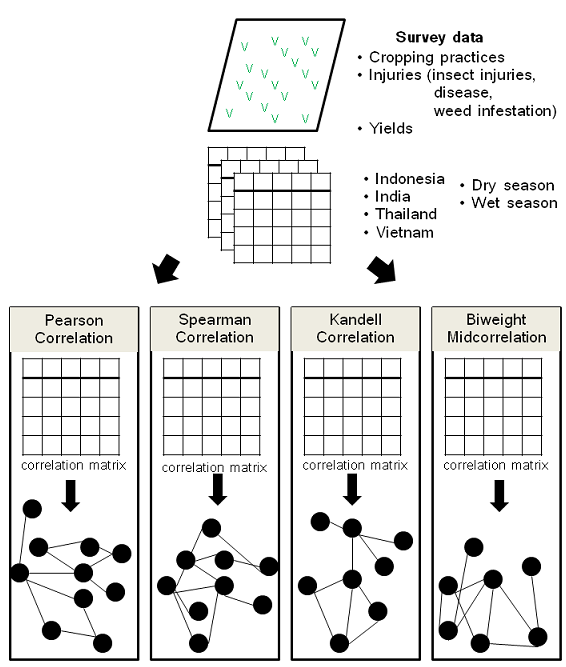
\includegraphics[resolution = 600]{pipeline}
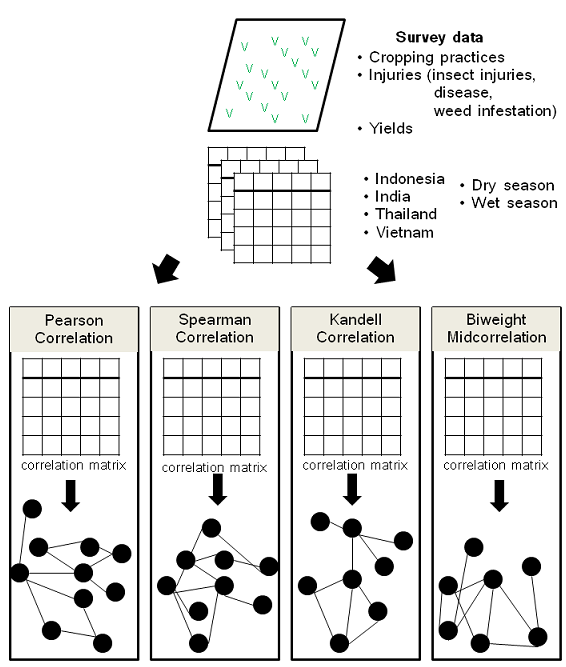
\includegraphics[width=6in]{pipeline}

\caption[Proposed pipeline for network construction]{Proposed pipeline for network construction. (a) Collect the input profiling data and output profiling data from different samples and different locations. (b) Calculate correlation coefficients (Pearson, Spearman, or Kendall). Estimate P-values for all coefficients. Next, determine threshold values for the resulting correlation coefficients and \textit{P} values, storing results in adjacency matrices for the construction of networks. (c) Construct network and analyze network for graph-theoretic properties and infer biological meanings and integrate the network of input data and output data. (d) Repeat analysis for a second season to verify the network model.}
\label{fig:pipeline}
\end{figure}
\end{landscape}

\newpage
\begin{landscape}
\begin{figure}[h!]
\centering
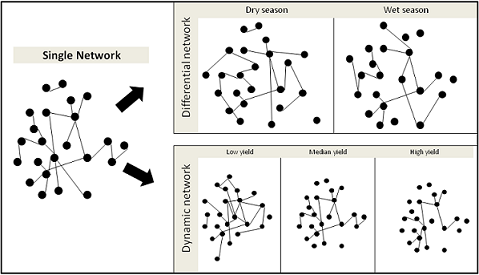
\includegraphics[width=6in]{wholenet}

\caption[Network comparison]{Network comparison: Network models constructed from survey datasets of different geographic locations are compared by determining their properties. Networks will express the conserved domains within their structure. A merged representation of the two networks being compared is also proposed as a holistic network of rice ecosystem in South and South East Asia.}
\label{fig:wholenet}
\end{figure}
\end{landscape}




%=============================================
% CONCLUSION
%\chapter{Conclusion}
%==============================================
%%===================
% CONCLUSION
%===================
To manage broad range of pests in sustainable way of agriculture, understandings of yield constrains are required priority. Agroecosystems are diverse and complex. Networks are commonly applied to analyze systemic interplay of biological components. Network analysis enables us to the explore the complex biological process and understand holistically. The gene-gene interaction networks, for instance, reveal the gene functions and system. Besides, the emergence properties after network reconstruction give the clues to cluster the components that close related, called hub. Networks are not static when different environment can reprogram the components arrangements and functions. Moreover, networks can allow us the consider the only the elements response the given changes. With versatile applications of network analysis, agroecosystem potentially can be modeled as a network. The new type of information will be proposed from the network analysis. One of the most challenge will be the model evaluation. Because this is the first attempt to applied network into the context of rice agroecosystem. Meeting this goal will require the development the validated methods to integrate heterogeneous data and built different networks on the basis of the particular rice agroecosystem.   




% The \appendix statement indicates the beginning of the appendices.

%----------------------------------------------------------------------
% END MATERIAL
%----------------------------------------------------------------------

% B I B L I O G R A P H Y
% -----------------------

\renewcommand{\bibname}{LITERATURE CITED}
\bibliographystyle{apacite}
\bibliography{sith-outline}
\end{document}
`